\chapter{%
    Regelbarkeit und Stabilisierbarkeit%
}

\section{%
    Regelbarkeit und die \name{Kalman}-Matrix%
}

Gegeben seien ein LTI-System $\dot{x} = Ax + Bu$, $x(0) = \xi \in \real^n$
mit $A \in \real^{n \times n}$ und $B \in \real^{n \times m}$
sowie ein fester Zeitpunkt $T > 0$.
Im Folgenden soll untersucht werden, welche Zustände zur Zeit $T$ erreicht werden können,
indem man eine geeignete Steuergröße $u(\cdot)$ verwendet.

Weil $x(T) = e^{AT} \xi + \int_0^T e^{A(T - \tau)} Bu(\tau) \d\tau$ gilt
und der erste Summand nicht von $u(\cdot)$ abhängt, reicht es aus, die möglichen Werte
von $\int_0^T e^{A(T - \tau)} Bu(\tau)\d\tau$ zu analysieren
(also für $\xi = 0$).

\textbf{erreichbare Menge}:
Die \begriff{erreichbare Menge (reachable set)} $\R_T$ von $\dot{x} = Ax + Bu$ zur Zeit $T > 0$
ist die Menge aller Zustände $x(T)$, die vom Null-Anfangswert durch einen stetigen Steuereingang
erreicht werden können,
also $\R_T := \left\{\left.\int_0^T e^{A(T - \tau)} Bu(\tau)\d\tau \;\right|
u \in \C([0, T], \real^m)\right\}$.

\linie

Zunächst benötigt man ein paar Definitionen aus der linearen Algebra.
Sei dazu $A \in \real^{n \times p}$.

\textbf{Bildraum}:
Der \begriff{Bildraum (range space)} $R(A) := \{Ax \;|\; x \in \real^p\}$ ist die Menge
aller Linearkombinationen der Spalten von $A$.

\textbf{Nullraum}:
Der \begriff{Nullraum (null space)} oder \begriff{Kern} ist
$N(A) := \{x \in \real^p \;|\; Ax = 0\}$.

\textbf{Zeilen-/Spaltenrang}:
Es gilt $R(A) = \real^n$ genau dann, wenn $A$ vollen Zeilenrang hat.\\
Es gilt $N(A) = \{0\}$ genau dann, wenn $A$ vollen Spaltenrang hat.

\textbf{orthogonales Komplement des Bilds}:
Es gilt $N(A^T) = R(A)^\bot$.

\textbf{\name{Cayley}-\name{Hamilton}}:
Für $A \in \real^{n \times n}$ quadratisch und $k \in \natural_0$
ist die $k$-te Potenz $A^k$ eine Linearkombination von $I, A, \dotsc, A^{n-1}$,
da $\chi_A(A) = 0$ mit $\chi_A$ dem charakteristischen Polynom von $A$.

\linie

\textbf{Beobachtung}:
Für $u \in \C([0, T], \real^m)$ gilt, dass
$x(T) = \int_0^T e^{A(T-\tau)} B u(\tau) \d\tau = \lim_{N \to \infty} x_N$
mit $x_N := \int_0^T \sum_{k=0}^N \frac{1}{k!} [A(T - \tau)]^k Bu(\tau)\d\tau$,
weil die Potenzreihe des Matrixexponentials gleichmäßig konvergiert.
$x_N$ lässt sich umschreiben zu
$x_N = \sum_{k=0}^N A^k B \cdot \left[\int_0^T \frac{(T - \tau)^k}{k!} u(\tau)\d\tau\right]$.
Der Ausdruck in eckigen Klammern ist ein Vektor $v_k \in \real^m$,
d.\,h. $x_N$ ist eine Linearkombination der Spalten von $B, AB, \dotsc, A^N B$.
Weil alle Matrizen $A^n, A^{n+1} B, \dotsc, A^N B$ wegen Cayley-Hamilton
Linearkombinationen von den Matrizen $B, AB, \dotsc, A^{n-1} B$ sind,
ist $x_N$ für alle $N \in \natural_0$ eine Linearkombination der Spalten
von $B, AB, \dotsc, A^{n-1} B$
d.\,h. $x_N \in R\smallpmatrix{B & AB & \cdots & A^{n-1} B}$.
Im Grenzübergang gilt daher auch $x(T) \in R\smallpmatrix{B & AB & \cdots & A^{n-1} B}$,
weil $R\smallpmatrix{B & AB & \cdots & A^{n-1} B}$ als endlich-dimensionaler Unterraum
topologisch abgeschlossen ist.

\textbf{\name{Kalman}-Matrix}:
Die \begriff{\name{Kalman}-Matrix} oder \begriff{Regelbarkeitsmatrix (controllability matrix)}
für das lineare System
$\dot{x} = Ax + Bu$ (oder das Paar $(A, B)$) ist definiert durch
$K := \smallpmatrix{B & AB & \cdots & A^{n-1} B}$.

Gerade wurde gezeigt, dass $\R_T \subset R(K)$.
Allerdings gilt sogar Gleichheit.

\linie
\pagebreak

\textbf{Regelbarkeits-\name{Gram}-Matrix}:
Die \begriff{Regelbarkeits-\name{Gram}-Matrix (controllability \name{Gram}ian)} von\\
$(A, B)$ zur Zeit $T > 0$ ist
$W_T := \int_0^T e^{At} BB^T e^{A^Tt}\dt =
\int_0^T e^{A(T-\tau)} BB^T e^{A^T(T-\tau)}\d\tau \in \real^{n \times n}$.

Weil die Einträge von $e^{At} BB^T e^{A^Tt}$ Linearkombinationen von Termen der Form
$t^k e^{\lambda t}$ sind, kann man $W_T$ explizit ausrechnen.

\textbf{Lemma}:
$W_T$ ist symmetrisch und positiv semidefinit.
Außerdem gilt $R(W_T) = R(K)$.

\textbf{Konstruktion von Steuergrößen}:
Sei $x_f \in R(K)$ beliebig.
Dann gibt es nach dem Lemma ein $\alpha \in \real^n$ mit $x_f = W_T \alpha$.
Mit der Steuergröße $u(\tau) := B^T e^{A^T (T - \tau)} \alpha$ erhält man\\
$x(T) = \int_0^T e^{A(T - \tau)} Bu(\tau) \d\tau
= \int_0^T e^{A(T - \tau)} B B^T e^{A^T (T - \tau)} \alpha \d\tau
= W_T \alpha = x_f$.
Also steuert diese Steuergröße vom Nullzustand in den Zustand $x_f$ zur Zeitpunkt $T$,
d.\,h. $x_f \in \R_T$.
Daher gilt auch die Umkehrung der obigen Inklusion: $R(K) \subset \R_T$.

\linie

\textbf{Satz (erreichbare Menge ist das Bild der Kalman-Matrix)}:\\
Es gilt $\R_T = R(K)$ mit der Kalman-Matrix
$K := \smallpmatrix{B & AB & \cdots & A^{n-1} B}$.

Daher ist $\R_T$ ein Unterraum von $\real^n$, der sogar unabhängig von $T > 0$ ist.
Man schreibt deswegen $\R := R(K)$.

\textbf{regelbar}:
Das lineare System $\dot{x} = Ax + Bu$ (oder das Paar $(A, B)$) heißt
\begriff{regelbar (controllable)}, falls $\R = \real^n$.

\textbf{Satz (\name{Kalman}-Test zur Regelbarkeit)}:
Das System definiert durch $(A, B)$ ist regelbar genau dann,
wenn die Kalman-Matrix $K := \smallpmatrix{B & AB & \cdots & A^{n-1} B}$ vollen Zeilenrang hat.

\section{%
    Punkt-zu-Punkt-Regelung%
}

Wenn man versucht, $x_f \in \real^n$ von einem Anfangswert $\xi \in \real^n$ mit $\xi \not= 0$
zu erreichen, dann muss eine Steuergröße $u(\cdot)$ gefunden werden,
sodass gilt:
$x_f = e^{AT}\xi + \int_0^T e^{A(T-\tau)} Bu(\tau) \d\tau$,
d.\,h. $x_f - e^{AT}\xi \in \R$.

\textbf{Satz (Punkt-zu-Punkt-Regelung)}:
Der Zustand $x(0) = \xi$ kann in den Zustand $x(T) = x_f$ ($T > 0$) geregelt werden genau dann,
wenn $x_f - e^{AT} \xi \in R(K)$.

Durch die Beweise kann man die notwendige Steuergröße $u(\cdot)$ sogar explizit angeben.

\textbf{Folgerung}:
Bei regelbaren Systemen kann man von jedem Anfangszustand $\xi \in \real^n$
zur Zeit $0$ zu jedem Endzustand $x_f \in \real^n$ zur Zeit $T > 0$ steuern.

\textbf{Bemerkung}:
Falls $A$ invertierbar ist und $(x_1, u_1)$, $(x_2, u_2)$ Gleichgewichte von
$\dot{x} = Ax + Bu$ sind, dann kann man von $x_1$ zu $x_2$ steuern,\\
denn $x_2 \in R(K)$
(nach Cayley-Hamilton gilt $A^{-1} = -\frac{1}{\alpha_n} (A^{n-1} + \alpha_1 A^{n-2} + \dotsb +
\alpha_{n-1} I)$ mit $\chi_A(\lambda) = \lambda^n + \alpha_1 \lambda^{n-1} + \dotsb + \alpha_n$,
daraus folgt $x_2 = -A^{-1} Bu_2 \in R(K)$)\\
und $e^{AT} x_1 \in R(K)$
(da $e^{AT} x_1 = \sum_{k=0}^\infty \frac{T^k}{k!} (A^k x_1)$
mit $A^k x_1 \in R(K)$, weil $x_1 \in R(K)$ und $R(K)$ $A$-invariant ist,
daraus folgt $e^{AT} x_1 \in R(K)$, weil $R(K) \subset \real^n$ abgeschlossen ist).\\
Somit ist $x_2 - e^{AT} x_1 \in R(K)$.

\pagebreak

\section{%
    Eigenschaften der \name{Kalman}-Matrix%
}

\textbf{Satz (geometrische Charakterisierung von $\R$)}:\\
$\R = R(K)$ ist der kleinste $A$-invariante Teilraum, der $R(B)$ enthält.

\linie

Die Zustandskoordinaten-Transformation $z = Tx$ des
Systems $\dot{x} = Ax + Bu$, $y = Cx + Du$ mit $T$ invertierbar führt zu
$\dot{z} = \widetilde{A} z + \widetilde{B} u$, $y = \widetilde{C} z + \widetilde{D} u$
mit $\smallpmatrix{\widetilde{A} & \widetilde{B} \\ \widetilde{C} & \widetilde{D}}
:= \smallpmatrix{TAT^{-1} & TB \\ CT^{-1} & D}$.
Man sieht schnell, dass die Kalman-Matrix $\widetilde{K}$ des transformierten Systems
bestimmt ist durch $\widetilde{K} := TK$, wobei $K$ die Kalman-Matrix von $(A, B)$ ist.

\textbf{Lemma (Koordinatentransformation)}:
Die Kalman-Matrizen $K$ von $(A, B)$ und $\widetilde{K}$ von $(\widetilde{A}, \widetilde{B})$
hängen zusammen durch $\widetilde{K} = TK$.
Daher ist Regelbarkeit invariant unter Zustandskoor"-dinaten-Transformation.

\section{%
    Regelbar-kanonische Form (SI-Systeme)%
}

\textbf{SI-System}:
Ein \begriff{SI-System (single-input system)} ist ein System $\dot{x} = Ax + Bu$ mit $m = 1$.

\linie

\textbf{regelbar-kanonische Form}:
Ein SI-System $\dot{x} = \widetilde{A}x + \widetilde{B}u$ mit\\
einer \begriff{Begleitmatrix}
$\widetilde{A} := \smallpmatrix{-\alpha_1 & -\alpha_2 & \cdots & -\alpha_n \\
1 & 0 & & & \\ & \ddots & \ddots & & \\ 0 & & 1 & 0}$
und dem ersten \begriff{Einheitsvektor} $\widetilde{B} := \smallpmatrix{1 \\ 0 \\ \vdots \\ 0}$\\
heißt in \begriff{regelbar-kanonischer Form (controllable canonical form)}
oder \begriff{RKF}.

SI-Systeme treten oft auf.
Insbesondere die regelbar-kanonische Form erhält man direkt, wenn
man eine DGL höheren Grades in ein System erster Ordnung umformt.
Die Kalman-Matrix $\widetilde{K}$ von $(\widetilde{A}, \widetilde{B})$ ist
eine quadratische, obere Dreiecksmatrix
$\widetilde{K} = \smallpmatrix{1 & -\alpha_1 & \ast & \cdots & \ast \\
& 1 & -\alpha_1 & \cdots & \ast \\ & & \ddots & \ddots & \vdots \\ & & & 1 & -\alpha_1 \\
0 & & & & 1}$ mit Einsen auf der Diagonalen.
Daher ist sie für alle $\alpha_1, \dotsc, \alpha_n \in \real$ invertierbar.

\textbf{Lemma (RKF ist regelbar)}:\\
Jede regelbar-kanonische Form $(\widetilde{A}, \widetilde{B})$ ist regelbar.

\linie

\textbf{Satz (jedes regelbare SI-System kann in RKF gebracht werden)}:\\
Für jedes regelbare SI-System $\dot{x} = Ax + Bu$ (also $m = 1$)
gibt es eine Koordinatentransformation $z = Tx$ mit $T$ invertierbar,
sodass $\dot{z} = [TAT^{-1}] z + [TB] u$ in regelbar-kanonischer Form ist.

Der Beweis ist konstruktiv:
Wenn $s_1, \dotsc, s_n$ die Spalten von $S = T^{-1} = \smallpmatrix{s_1 & \cdots & s_n}$ sind,
dann muss $B = S\widetilde{B}$ und $AS = S\widetilde{A}$ mit $(\widetilde{A}, \widetilde{B})$
in RKF (siehe oben) gelten.
Aus der ersten Gleichung erhält man $s_1 := B$.
Induktiv setzt man in die zweite Gleichung ein, um\\
$s_2 := (A + \alpha_1 I) B$,
$s_3 := (A^2 + \alpha_1 A + \alpha_2 I) B$, \dots,
$s_n := (A^{n-1} + \alpha A^{n-1} + \dotsb + \alpha_{n-1} I) B$
zu erhalten.
Etwas zusätzliche Argumentation ist noch nötig
(z.\,B. warum $S$ invertierbar ist).

\linie

Weil sich das charakteristische Polynom in der RKF sofort ablesen lässt
(nämlich\\
$\chi_{\widetilde{A}}(\lambda) = \lambda^n + \alpha_1 \lambda^{n-1} + \dotsb + \alpha_n$)
und ähnliche Matrizen dasselbe charakteristische Polynom besitzen,
lässt sich die regelbar-kanonische Form von $(A, B)$
direkt angeben und ist eindeutig.

\pagebreak

\section{%
    Regelbarkeits-Normalform (MI-Systeme)%
}

Im Folgenden geht es hauptsächlich um MI-Systeme, die Sätze lassen sich aber auch auf SI-Systeme
anwenden.

\textbf{MI-System}:
Ein \begriff{MI-System (multi-input system)} ist ein System $\dot{x} = Ax + Bu$ mit $m > 1$.

\linie

\textbf{Unregelbarkeit}:
Unregelbarkeit kann viele Ursachen haben.
Durch Verbindung von regelbaren System (Parallel-, Reihenschaltung, Rückführung)
kann Regelbarkeit zerstört werden -- muss aber nicht.
Eine mögliche Situation tritt auf,
wenn zwei identische regelbare Systeme $\dot{x}_S = A_S x_S + B_S u$ mit demselben
Eingang gesteuert werden,
d.\,h. $\dot{x} = Ax + Bu$ mit $A := \smallpmatrix{A_S & 0 \\ 0 & A_S}$ und
$B := \smallpmatrix{B_S \\ B_S}$.
Die Kalman-Matrix von $(A, B)$ hat keinen vollen Zeilenrang, weil sie gleich
$\smallpmatrix{B_S & A_S B_S & \cdots & A_S^{n-1} B_S \\ B_S & A_S B_S & \cdots & A_S^{n-1} B_S}$
ist.
Die erreichbare Menge von $(A, B)$ ist gleich
$\left\{\left.\smallpmatrix{x \\ x} \;\right|\; x \in \real^n\right\}$.

\linie

\textbf{Herleitung der RNF}:
Falls $\dot{x} = Ax + Bu$ nicht regelbar ist, dann gilt $n_1 := \rg(K) < n$
bzw. $n_2 := n - n_1 > 0$.
Fasst man $n_1$ linear unabhängige Spalten von $K$ in der Matrix $S_1 \in \real^{n \times n_1}$
zusammen, so kann man diese mit $n_2$ Vektoren, die in der Matrix $S_2 \in \real^{n \times n_2}$
zusammengefasst werden, zu einer Basis von $\real^n$ ergänzen.
Die invertierbare Matrix $S := \smallpmatrix{S_1 & S_2} \in \real^{n \times (n_1 + n_2)}$
kann man zur Zustandskoordinaten-Transformation verwenden.

\textbf{Struktur der RNF}:
Es gilt $\widetilde{A} := S^{-1} AS = \smallpmatrix{A_{11} & A_{12} \\ 0 & A_{22}}$
und $\widetilde{B} := S^{-1} B = \smallpmatrix{B_1 \\ 0}$ mit\\
$A_{11} \in \real^{n_1 \times n_1}$, $A_{22} \in \real^{n_2 \times n_2}$ und
$B_1 \in \real^{n_1 \times m}$.
Außerdem ist $(A_{11}, B_1)$ regelbar.

\textbf{Satz (Regelbarkeits-Normalform)}:
Für jedes lineare System $\dot{x} = Ax + Bu$ gibt es eine Zustands"-koordinaten-Transformation,
die das System in das System\\
$\smallpmatrix{\dot{z}_1 \\ \dot{z}_2} =
\smallpmatrix{A_{11} & A_{12} \\ 0 & A_{22}} \smallpmatrix{z_1 \\ z_2} +
\smallpmatrix{B_1 \\ 0} u$ transformiert,
wobei $(A_{11}, B_1)$ regelbar ist.\\
Diese Form heißt
\begriff{Regelbarkeits-Normalform (controllability normal form)} oder \begriff{RNF}.

Ausgeschrieben bedeutet das $\dot{z}_1 = A_{11} z_1 + A_{12} z_2 + B_1 u$,
$\dot{z}_2 = A_{22} z_2$.
Somit kann $z_2(\cdot)$ nicht durch die Steuergröße beeinflusst werden.

\textbf{unregelbare Eigenwerte}:\\
Die Eigenwerte von $A_{22}$ heißen \begriff{unregelbare Eigenwerte (uncontrollable modes)}
von $(A, B)$.

Mit $z_1(0) = z_1^0$ gilt
$z_1(t) = e^{A_{11}t} z_1^0 + \int_0^t e^{A_{11}(t - \tau)} \smallpmatrix{A_{12} & B_1}
\smallpmatrix{z_2(\tau) \\ u(\tau)} \d\tau$,
wenn man $z_2$ und $u$ in einem Eingang zusammenfasst.
Indem man $z_2(t) = e^{A_{22}t} z_2^0$ ($z_2(0) = z_2^0$) einsetzt, erhält man
die Lösung
$z_1(t) = e^{A_{11}t} \left(z_1^0 +
\left[\int_0^t e^{-A_{11}\tau} A_{12} e^{A_{22}\tau} \d\tau\right] z_2^0\right) +
\int_0^t e^{A_{11}(t - \tau)} B_1 u(\tau) \d\tau$.
Weil $(A_{11}, B_1)$ regelbar ist, kann man den Zustand $z_1$ von jedem Anfangzustand
$z_1^0$ zur Zeit $0$ in jeden Endzustand $z_1^f$ zur Zeit $T > 0$ regeln,
wenn man von $z_1^0$ vorher den "`Störterm"' $[\cdots]z_2^0$ abzieht.

\linie

\textbf{Links-Eigenvektor}:\\
$e$ ist ein \begriff{Links-Eigenvektor} einer Matrix $A$, falls
$e \not= 0$ und $e^\ast (A - \lambda I) = 0$ mit $e^\ast := \overline{e}^T$.

\textbf{Satz (\name{Hautus}-Test zur Regelbarkeit)}:
$(A, B)$ ist regelbar genau dann, wenn für
jeden Links-Eigenvektor $e$ von $A$ gilt, dass $e^\ast B \not= 0$.
Äquivalent dazu ist, dass die Matrix $\smallpmatrix{A - \lambda I & B}$
vollen Zeilenrang für alle $\lambda \in \complex$ besitzt.

Wegen $S^{-1} \smallpmatrix{A - \lambda I & B} \smallpmatrix{S & 0 \\ 0 & I} =
\smallpmatrix{\widetilde{A} - \lambda I & \widetilde{B}}$ und
$\rg\smallpmatrix{A_{11} - \lambda I & B_1} = n_1$
(d.\,h. voller Zeilenrang) für alle $\lambda \in \complex$ gilt
$\rg\smallpmatrix{A - \lambda I & B}
= \rg\smallpmatrix{\widetilde{A} - \lambda I & \widetilde{B}}
= n_1 + \rg(A_{22} - \lambda I)$
für alle $\lambda \in \complex$,
also folgendes Korollar,
mit dem sich die unregelbaren Eigenwerte ohne Berechnung der RNF bestimmen lassen.

\textbf{Folgerung}:
Die unregelbaren Eigenwerte von $(A, B)$ sind gegeben durch\\
$\left\{\lambda \in \complex \;\left|\; \rg\smallpmatrix{A - \lambda I & B} < n\right.\right\}$.

\pagebreak

\section{%
    Stabilisierbarkeit%
}

Stabilisierbarkeit ist eine Verallgemeinerung von Regelbarkeit.
Regelbarkeit von $\dot{x} = Ax + Bu$ impliziert, dass jeder Anfangszustand
in einem endlichen Zeitintervall zur $0$ gesteuert werden kann
(sogar in jedem beliebig kleinen Intervall).
Bei Stabilisierbarkeit verlangt man dies nur noch asymptotisch für $t \to \infty$.

\textbf{Stabilisierbarkeit}:
Das lineare System $\dot{x} = Ax + Bu$ (oder das Paar $(A, B)$) heißt
\begriff{stabilisierbar (stabilizable)}, falls
für jeden Anfangszustand $\xi \in \real^n$ eine stückweise stetige Steuergröße\\
$u\colon [0, \infty) \rightarrow \real^m$ existiert, sodass $\lim_{t \to \infty} x(t) = 0$
für $x(0) = \xi$.

Jedes regelbare System ist stabilisierbar:
Wähle $T > 0$ beliebig.
Wenn $u_T(\cdot)$ die Steuergröße ist, die von $x(0) = \xi$ zu $x(T) = 0$ steuert,
dann ist $u(t) := u_T(t)$ für $t \le T$ und $u(t) := 0$ für $t > T$ eine
stabilisierende Steuergröße, da $\dot{x} = Ax + Bu = 0$ für $x = u = 0$,
also $x(t) = 0$ für $t > T$.

\linie

\textbf{\name{Hautus}-Test zur Stabilisierbarkeit}:
$(A, B)$ ist stabilisierbar genau dann, wenn
die unregelbaren Eigenwerte alle negative Realteile besitzen.
Äquivalent dazu ist, dass $\smallpmatrix{A - \lambda I & B}$ vollen Zeilenrang für alle
$\lambda \in \complex$ mit $\Re(\lambda) \ge 0$ besitzt.

Dabei reicht es natürlich, nur die Eigenwerte $\lambda$ von $A$ mit nicht-negativem Realteil
zu betrachten.
Wenn $A$ eine Hurwitz-Matrix ist, dann ist $\dot{x} = Ax + Bu$ stabilisierbar
(mit $u(t) \equiv 0$).

\section{%
    Of"|fene und geschlossene Regelkreise%
}

\textbf{of"|fene Regelkreise}:
Bisher wurden nur \begriff{of"|fene Regelkreise (open-loop control)} betrachtet,
die durch eine A-priori-Steuergröße $u(t)$ für $t \ge 0$ gesteuert werden.
Das geregelte System wird durch $\dot{x}(t) = Ax(t) + Bu(t)$ mit $x(0) = \xi$ beschrieben.
Dieser Ansatz besitzt einige Nachteile:
\begin{itemize}
    \item
    Für verschiedene Anfangsbedingungen müssen verschiedene Steuergrößen gewählt werden,
    um die Aufgabenstellung zu erfüllen.
    Die Steuergrößen müssen "`manuell"' an den jeweiligen Anfangszustand angepasst werden.

    \item
    Zukünftige, unvorhergesehene Ereignisse werden nicht berücksichtigt.
    Strategien mit of"|fenen Regelkreisen sind vorgeplant und passen sich nicht Situationen an,
    in denen das System sich nicht gewünscht verhält, d.\,h. sie sind nicht robust.
\end{itemize}

\linie

\textbf{geschlossene Regelkreise (Rückführung)}:
In einem \begriff{geschlossenen Regelkreis} empfängt ein
\begriff{Rückführungsregler (feedback controller)} Informationen vom System,
verarbeitet diese und erzeugt ein Steuersignal, das zurück zum System gesendet wird.
Man kann dies wie folgt grafisch veranschaulichen:

\begin{center}
    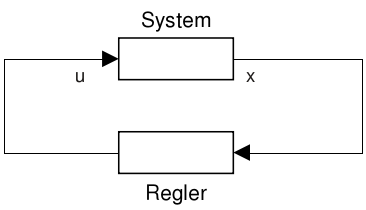
\includegraphics[scale=\modelscale]{rueckkopplung}
\end{center}

\pagebreak

\section{%
    Polvorgabe%
}

\textbf{Regelung durch lineare Zustandsrückführung}:
Bei einem System mit $x$-Dimension $n$ und $u$-Dimension $m$ ist
der \begriff{lineare Zustandsrückführungs-Regler (linear state-feedback controller)} definiert
durch $u = -Fx$ mit $F \in \real^{m \times n}$.

Für ein LTI-System $\dot{x} = Ax + Bu$ führt dies zu
$\dot{x} = Ax - BFx = (A - BF)x$
(\begriff{geschlossener Regelkreis (closed-loop system)} oder
\begriff{geregeltes System}).
Der Regler verändert daher die Dynamik des Systems vom ungeregelten System
$\dot{x} = Ax$ zum geregelten System $\dot{x} = (A - BF)x$.
Eine andere Interpretation ist, dass der Regler zur Zeit $t$ den Zustand $x(t)$ misst und
die Steuergröße $u(t) = -Fx(t)$ durch Bildung von Linearkombinationen der
Einträge von $x(t)$ berechnet.

\linie

Die Eigenwerte des Systems $\dot{x} = (A - BF)x$ bestimmen das
Verhalten des Systems.
Umso erstaunlicher ist es, dass bei regelbaren Systemen die Matrix $F$ stets so gewählt werden
kann, dass $A - BF$ beliebig vorgegebene Eigenwerte besitzt.
Weil diese eine Obermenge der Polstellen der Übertragungsmatrix darstellen, spricht man auch von
\begriff{Polvorgabe (pole placement)}.

\textbf{Satz (Polvorgabe)}:
Sei $(A, B)$ regelbar mit $A \in \real^{n \times n}$ und $B \in \real^{n \times m}$.\\
Wenn $\lambda_1, \dotsc, \lambda_n \in \complex$ (nicht notwendigerweise paarweise verschieden)
symmetrisch bzgl. der reellen Achse sind, dann gibt es eine Matrix $F \in \real^{m \times n}$
mit $\Eig(A - BF) = \{\lambda_1, \dotsc, \lambda_n\}$.

\linie

\textbf{Beweis für SI-Systeme}:
Ist $m = 1$, dann lässt sich $(A, B)$ in RKF bringen, d.\,h.\\
$\widetilde{A} = \smallpmatrix{-\alpha_1 & -\alpha_2 & \cdots & -\alpha_n \\
1 & 0 & & & \\ & \ddots & \ddots & & \\ 0 & & 1 & 0}$,
$\widetilde{B} = \smallpmatrix{1 \\ 0 \\ \vdots \\ 0}$ und
$\widetilde{A} - \widetilde{B} \widetilde{F} =
\smallpmatrix{-\alpha_1 - \widetilde{f}_1 & -\alpha_2 - \widetilde{f}_2 & \cdots &
-\alpha_n - \widetilde{f}_n \\
1 & 0 & & & \\ & \ddots & \ddots & & \\ 0 & & 1 & 0}$\\
mit $\widetilde{A} = TAT^{-1}$ und $\widetilde{B} = TB$ für $T \in \GL_n(\real)$ und
$\widetilde{F} = \smallpmatrix{\widetilde{f}_1 & \cdots & \widetilde{f}_n}
\in \real^{1 \times n}$.
Damit gilt\\
$\chi_{\widetilde{A} - \widetilde{B} \widetilde{F}}(s) =
s^n + (\alpha_1 + \widetilde{f}_1) s^{n-1} + \dotsb + (\alpha_n + \widetilde{f}_n)$.
Durch Wahl von $\widetilde{F}$ kann $\chi_{\widetilde{A} - \widetilde{B} \widetilde{F}}$
jedes beliebige reelle, normierte Polynom $n$-ten Grades sein,
also auch $(s - \lambda_1) \dotsm (s - \lambda_n)$.
Für $F := \widetilde{F} T$ gilt dann
$\widetilde{A} - \widetilde{B} \widetilde{F} = TAT^{-1} - TBFT^{-1} = T(A - BF)T^{-1}$,
somit $\chi_{A - BF} = \chi_{\widetilde{A} - \widetilde{B} \widetilde{F}}$.

Wenn man sich die Konstruktion von $S = T^{-1}$ im Beweis zur regelbar-kanonischen Form anschaut,
dann sieht man, dass $S = K T_\alpha$ mit
$K := \smallpmatrix{B & AB & \cdots & A^{n-1} B}$ der Kalman-Matrix und
$T_\alpha := \smallpmatrix{1 & \alpha_1 & \alpha_2 & \cdots & \alpha_{n-1} \\
& 1 & \alpha_1 & \cdots & \alpha_{n-2} \\
& & 1 & \cdots & \alpha_{n-3} \\
& & & \ddots & \vdots \\
0 & & & & 1}$.
Daher muss man $F = \smallpmatrix{\widetilde{f}_1 & \cdots & \widetilde{f}_n} [K T_\alpha]^{-1}$
wählen, wenn das charakteristische Polynom von $A - BF$ die Koef"|fizienten
$\alpha_1 + \widetilde{f}_1$, \dots, $\alpha_n + \widetilde{f}_n$ haben soll
(\begriff{\name{Bass}-\name{Gura}-Formel} oder \begriff{alternative \name{Ackermann}-Formel}).

\linie

\textbf{Beweis für MI-Systeme}:
Für den Beweis für $m > 1$ benötigt man zwei Lemmata.

\textbf{Lemma}:
Für $(A, B)$ regelbar
gibt es für alle $b \in R(B) \setminus \{0\}$ Vektoren $u_1, \dotsc, u_{n-1} \in \real^m$,
sodass $\{x_1, \dotsc, x_n\}$ linear unabhängig ist, wobei die $x_i$ definiert sind
durch $x_1 := b$ und die Rekursion $x_{i+1} := Ax_i + Bu_i$,
$i = 1, \dotsc, n - 1$.

Der Beweis erfolgt per Induktion:
Wegen $x_1 = b \not= 0$ ist $\{x_1\}$ l.u.
Seien $x_1, \dotsc, x_k$ l.u. mit $k < n$ und $V := [x_1, \dotsc, x_k]$.
Zeige $Ax_k + Bu_k \notin V$ für ein $u_k \in \real^m$ durch Widerspruch:
Angenommen, für alle $u \in \real^m$ gilt $Ax_k + Bu \in V$.
Dann gilt insbesondere $Ax_k \in V$ und somit $Bu \in V$ für alle $u \in \real^m$,
d.\,h. $R(B) \subset V$.
Damit gilt $Ax_i = x_{i+1} - Bu_i \in V$ für alle $i = 1, \dotsc, k - 1$,
zusätzlich gilt $Ax_k \in V$.
$V$ ist also $A$-invariant und enthält $R(B)$, d.\,h. $\real^n = R(K) \subset V$
aufgrund $(A, B)$ regelbar, ein Widerspruch zu $\dim V = k < n$.

\linie
\pagebreak

\textbf{\name{Heymann}-Lemma}:
Für $(A, B)$ regelbar
gibt es für alle $b \in R(B) \setminus \{0\}$ eine Matrix $F \in \real^{m \times n}$,
sodass $(A + BF, b)$ regelbar ist.

Seien $u_1, \dotsc, u_{n-1} \in \real^m$ so gewählt, dass die $x_1, \dotsc, x_n$
aus dem vorherigen Lemma linear unabhängig sind.
Für $u_n := 0$ sei $F := \smallpmatrix{u_1 & \cdots & u_n} \cdot
\smallpmatrix{x_1 & \cdots & x_n}^{-1}$.
Dann ist $Fx_i = u_i$ und somit $x_{i+1} = Ax_i + Bu_i = (A + BF)x_i$ für $i = 1, \dotsc, n - 1$.
Man erhält also $x_i = (A + BF)^{i-1} x_1 = (A + BF)^{i-1} b$ für $i = 1, \dotsc, n$.
Die Matrix $\smallpmatrix{x_1 & \cdots & x_n}$ ist daher die Kalman-Matrix von $(A + BF, b)$,
weil sie invertierbar ist (Spalten linear unabhängig), ist $(A + BF, b)$ regelbar.

\linie

\textbf{Beweis für MI-Systeme}:
Mit dem Heymann-Lemma folgt der Satz über die Polvorgabe:
Wähle $b \in R(B) \setminus \{0\}$
(wenn $B$ die Nullmatrix wäre, dann wäre $(A, B)$ nicht regelbar).
Sei $\widetilde{F} \in \real^{m \times n}$ nach dem Heymann-Lemma, sodass
$(A + B\widetilde{F}, b)$ regelbar ist.
Wähle $\widehat{F} \in \real^{1 \times n}$, sodass
$\Eig((A + B\widetilde{F}) - b\widehat{F}) = \{\lambda_1, \dotsc, \lambda_n\}$
(geht nach dem schon bewiesenen Fall $m = 1$).
Wegen $b \in R(B)$ gibt es $u_0 \in \real^m$ mit $Bu_0 = b$.
Definiere $F := u_0 \widehat{F} - \widetilde{F}$.
Damit gilt $A - BF = A + B\widetilde{F} - Bu_0\widehat{F}
= A + B\widetilde{F} - b\widehat{F}$,
d.\,h. $A - BF$ besitzt die gewünschten Eigenwerte.

\linie

\textbf{unregelbare Systeme}:
Jedes System $(A, B)$ kann in Regelbarkeits-Normalform
$(\widetilde{A}, \widetilde{B})$ gebracht werden.
Wenn $\widetilde{F}$ eine Rückführungsverstärkung für das transformierte System ist,
dann können die Spalten von $\widetilde{F} = \smallpmatrix{\widetilde{F}_1 & \widetilde{F}_2}$
wie die von $\widetilde{A}$ eingeteilt werden.
Mit $u = -\widetilde{F}z$ erhält man das System
$\smallpmatrix{\dot{z}_1 \\ \dot{z}_2} = \smallpmatrix{A_{11} - B_1\widetilde{F}_1 &
A_{12} - B_1 \widetilde{F}_2 \\ 0 & A_{22}} \smallpmatrix{z_1 \\ z_2}$.
Weil $(A_{11}, B_1)$ regelbar ist, können die Eigenwerte von $A_{11} - B_1\widetilde{F}_1$
durch geeignete Wahl von $\widetilde{F}_1$ beliebig gewählt werden.
Daher wählt man $\widetilde{F}_1$ immer so, dass sie alle negativen Realteil haben.
Die Eigenwerte von $A_{22}$ kann man durch die lineare Zustandsregelung nicht beeinflussen,
was die Bezeichnung "`unregelbare Eigenwerte"' noch einmal rechtfertigt.
Für $(A, B)$ unregelbar gibt es also immer Eigenwerte von $A - BF$, die fest sind
und nicht durch $F$ verschoben werden können.

\linie

\textbf{Satz (Stabilisierung durch lineare Zustandsrückführung)}:
Das System $\dot{x} = Ax + Bu$ ist stabilisierbar genau dann, wenn
es eine Matrix $F \in \real^{m \times n}$ gibt, sodass $\dot{x} = (A - BF)x$
asymptotisch stabil ist (d.\,h. $A - BF$ ist eine Hurwitz-Matrix).

\section{%
    \emph{Zusatz}: Kanonische \name{Brunovsky}-Form%
}

\textbf{äquivalent}:
Die Paare $(A, B)$ und $(\widetilde{A}, \widetilde{B})$
(mit $A, \widetilde{A} \in \real^{n \times n}$ und
$B, \widetilde{B} \in \real^{n \times m}$) heißen \begriff{äquivalent},
falls es Matrizen $S \in \real^{n \times n}$ invertierbar, $U \in \real^{m \times m}$
invertierbar und $F \in \real^{m \times n}$ gibt, sodass
$S^{-1} \smallpmatrix{A & B} \smallpmatrix{S & 0 \\ -F & U} =
\smallpmatrix{\widetilde{A} & \widetilde{B}}$.

Man kann das auch schreiben als
$\widetilde{A} = S^{-1} AS - S^{-1} BF$ und $\widetilde{B} = S^{-1} BU$.
Äquivalent dazu kann man auch $-F$ durch $-FS$ ersetzen.
Äquivalenz von Paaren $(A, B)$ ist eine Äquivalenzrelation
auf der Menge $\real^{n \times n} \times \real^{n \times m}$ der Paare $(A, B)$.
$(\widetilde{A}, \widetilde{B})$ ist regelbar genau dann, wenn $(A, B)$ regelbar ist.

\textbf{Spezialfälle}:
\begin{enumerate}
    \item
    \emph{Zustandskoordinaten-Transformation} ($F = 0$, $U = I$):
    $\widetilde{A} = S^{-1} AS$ und $\widetilde{B} = S^{-1} B$\\
    (zugehöriges System $\dot{z} = S^{-1} ASz + S^{-1} Bu$)

    \item
    \emph{Eingangskoordinaten-Transformation} ($S = I$, $F = 0$):
    $\widetilde{A} = A$ und $\widetilde{B} = BU$\\
    (zugehöriges System $\dot{x} = Ax + BUv$ mit $u = Uv$)

    \item
    \emph{lineare Zustandsrückführung, neuer Eingang} ($S = I$, $U = I$):
    $\widetilde{A} = A - BF$ und $\widetilde{B} = B$\\
    (zugehöriges System $\dot{x} = (A - BF)x + Bv$ mit $u = -Fx + v$)
\end{enumerate}

\linie
\pagebreak

\textbf{Äquivalenz als Gruppenoperation}:
Wegen $\smallpmatrix{S_1 & 0 \\ -F_1 & U_1} \cdot \smallpmatrix{S_2 & 0 \\ -F_2 & U_2}
= \smallpmatrix{S_3 & 0 \\ -F_3 & U_3}$
mit $S_3 := S_1 S_2$ invertierbar, $U_3 = U_1 U_2$ invertierbar und
$F_3 := F_1 S_2 + U_1 F_2$ ist die Menge $G$ der
Blockmatrizen $\smallpmatrix{S & 0 \\ -F & U}$
mit $S$ und $U$ invertierbar eine Gruppe bzgl. der Multiplikation
(man braucht zusätzlich noch $\smallpmatrix{I & 0 \\ 0 & I} \in G$ und
$\smallpmatrix{S & 0 \\ -F & U}^{-1} = \smallpmatrix{S^{-1} & 0 \\ U^{-1}FS^{-1} & U^{-1}} \in G$).
Diese Gruppe definiert eine Gruppenoperation auf der Menge
$\real^{n \times n} \times \real^{n \times m}$ der Paare von Matrizen $(A, B)$:\\
$\smallpmatrix{S & 0 \\ -F & U} \cdot (A, B) := (\widetilde{A}, \widetilde{B})
= (S^{-1} AS - S^{-1} BF, S^{-1} BU)$.
Die Bahnen unter dieser Operation sind genau die Äquivalenzklassen der obigen Äquivalenz.

\linie

\textbf{Satz (kanonische \name{Brunovsky}-Form)}:
Sei $(A, B)$ regelbar, wobei $B \in \real^{n \times m}$ vollen Spaltenrang hat.
Dann gibt es $\kappa_1, \dotsc, \kappa_m \in \natural$ mit
$\kappa_1 \ge \dotsb \ge \kappa_m$
(\begriff{Regelbarkeits-Indizes (controllability indices)}),
sodass $(A, B)$ zu $(\widetilde{A}, \widetilde{B})$
äquivalent ist mit
\begin{align*}
    \widetilde{A} =
    \smallpmatrix{
        0 & 0 & \dotsb & 0 & & & & & 0 \\
        1 & 0 & & 0 & & & & & \\
        & \ddots & \ddots & \vdots & & & & & \\
        0 & & 1 & 0 & & & & & \\
        & & & & \ddots & & & & \\
        & & & & & 0 & 0 & \dotsb & 0 \\
        & & & & & 1 & 0 & & 0 \\
        & & & & & & \ddots & \ddots & \vdots \\
        0 & & & & & 0 & & 1 & 0
    },\quad
    \widetilde{B} =
    \smallpmatrix{
        1 & & 0 \\
        0 & & \\
        \vdots & & \\
        0 & & \\
        & \ddots & \\
        & & 1 \\
        & & 0 \\
        & & \vdots \\
        0 & & 0
    },
\end{align*}
wobei die Dimensionen der Kästchen $\kappa_i \times \kappa_i$ bzw. $\kappa_i \times 1$ sind
($i = 1, \dotsc, m$).\\
Diese Form heißt \begriff{kanonische \name{Brunovsky}-Form (\name{Brunovsky} canonical form)}.

Falls $B$ nicht vollen Spaltenrang hat, dann gibt es eine Eingangskoordinaten-Transformation
$Uv = u$ mit $U$ invertierbar, sodass $BU = \smallpmatrix{\widetilde{B}_1 & 0}$ gilt und
$\widetilde{B}_1$ vollen Spaltenrang hat.
In diesem Fall ist $Bu = BUv = \smallpmatrix{\widetilde{B}_1 & 0} \smallpmatrix{v_1 \\ v_2}
= \widetilde{B}_1 v_1$, d.\,h. der Teil $v_2$ des neuen Eingangs ist nicht relevant.
Daher nimmt man in der Literatur oft oBdA an, dass $B$ vollen Spaltenrang hat.

\textbf{\name{Brunovsky}-Form ohne lineare Zustandsregelung}:\\
Man kann obigen Satz auch ohne lineare Zustandsregelung formulieren (d.\,h. $F = 0$).\\
Es gibt eine Zustands- und Eingangskoordinaten-Transformation von $(A, B)$ in
$(\widetilde{A}, \widetilde{B})$ mit
\begin{align*}
    \widetilde{A} =
    \smallpmatrix{
        \ast & \ast & \cdots & \ast & \cdots & \cdots & \cdots & \cdots & \ast \\
        1 & 0 & & 0 & & & & & \\
        & \ddots & \ddots & \vdots & & & & & \\
        0 & & 1 & 0 & & & & & \\
        & & & & \ddots & & & & \\
        \ast & \cdots & \cdots & \cdots & \cdots & \ast & \ast & \cdots & \ast \\
        & & & & & 1 & 0 & & 0 \\
        & & & & & & \ddots & \ddots & \vdots \\
        0 & & & & & 0 & & 1 & 0
    },\quad
    \widetilde{B} =
    \smallpmatrix{
        1 & & 0 \\
        0 & & \\
        \vdots & & \\
        0 & & \\
        & \ddots & \\
        & & 1 \\
        & & 0 \\
        & & \vdots \\
        0 & & 0
    }.
\end{align*}

\linie

\textbf{Polvorgabe mit kanonischer \name{Brunovsky}-Form}:
Mit der kanonischen Brunovsky-Form ist der Satz über die Polvorgabe einfach zu zeigen
(allerdings ist der Satz über die kanonische Brunovsky-Form relativ aufwendig zu beweisen):
Für $\widetilde{F} \in \real^{m \times n}$ beliebig ist $\widetilde{B}\widetilde{F}$
eine $(n \times n)$-Matrix, die nur Nullen enthält, außer in den $\ast$-Zeilen von $\widetilde{A}$
(dort stehen die Zeilen von $\widetilde{F}$).
Somit kann man die Elemente von $\widetilde{F}$, die zu Einträgen von $\widetilde{A}$ außerhalb von
Blöcken gehören, so wählen, dass die $\ast$-Zeilen außerhalb der Blöcke $\widetilde{A}_i$
verschwinden.
Die übrigen Einträge von $\widetilde{F}$ (in den Blöcken $\widetilde{F}_i$) wählt man so, dass
$\widetilde{A}_i - \widetilde{B}_i \widetilde{F}_i$
die gewünschten Eigenwerte besitzt, was aufgrund der Polvorgabe für SI-Systeme möglich ist.
Damit besitzt auch $\widetilde{A} - \widetilde{B} \widetilde{F}$ die gewünschten Eigenwerte.
Wegen\\
$\widetilde{A} - \widetilde{B} \widetilde{F}
= S^{-1}AS - S^{-1}BF - S^{-1}BU \widetilde{F}
= S^{-1}AS - S^{-1}B(F + U\widetilde{F})
= S^{-1} (A - B\widehat{F}) S$
mit $\widehat{F} := (F + U\widetilde{F}) S^{-1}$
besitzt auch $A - B\widehat{F}$ die geforderten Eigenwerte.

\pagebreak

\section{%
    Dominante Eigenwerte%
}

\textbf{Dämpfungsverhältnis}:
Das \begriff{Dämpfungsverhältnis (damping ratio)} des nicht-reellen Eigenwerts
$\lambda \in \Eig(A) \setminus \real$ von $A$ ist definiert als
$\zeta := -\frac{\Re(\lambda)}{|\lambda|}$.

\textbf{dominanter Eigenwert}:
Ein Paar von nicht-reellen Eigenwerten $\lambda, \overline{\lambda} \in \Eig(A) \setminus \real$
von $A$ heißt \begriff{dominant}, falls ihr Dämpfungsverhältnis das kleinste aller
Dämpfungsverhältnisse von nicht-reellen Eigenwerten von $A$ ist.

Für Hurwitz-Matrizen $A$ ist das Verhalten von $t \mapsto e^{At}$ häufig (aber nicht immer)
hauptsächlich bestimmt durch den dominanten Eigenwert von $A$.
Wegen der reellen Jordan-Normalform von $A$ ist $e^{At}$ eine Überlagerung von $e$-Funktionen
mit reellen Exponenten oder von $e^{Jt}$ mit $(2 \times 2)$-Blöcken $J$ mit
nicht-reellen Eigenwerten.
Ist ein solcher Block $J$ eine Hurwitz-Matrix, dann bestimmt das Dämpfungsverhältnis die
Dominanz der Antwort.

\linie

\textbf{Platzierung der Eigenwerte}:
Diese Frage ist nicht leicht zu beantworten.
\begin{itemize}
    \item
    Die Bass-Gura-Formel
    $F = \smallpmatrix{\widetilde{f}_1 & \cdots & \widetilde{f}_n} [K T_\alpha]^{-1}$
    zeigt:
    Je kleiner die Verschiebung der Koef"|fizienten des charakteristischen Polynoms
    (und der Eigenwerte) ist, desto kleiner sind die Koef"|fizienten von $F$ --
    was wünschenswert ist, denn große Koef"|fizienten bedeuten einen großen Regelaufwand.

    \item
    Die Rolle von dominanten Eigenwerten führt zum folgenden Design-Rezept:
    \begin{itemize}
        \item
        Wähle ein System zweiter Ordnung mit der gewünschten Dynamik.

        \item
        Platziere zwei Eigenwerte an den zwei Polstellen des Systems.

        \item
        Wähle alle anderen Eigenwerte schneller (damit sie weniger dominant sind),
        aber nicht zu schnell (um zu starken Regelaufwand zu vermeiden).

        \item
        Platziere die Eigenwerte und überprüfe mittels dynamischer Simulation.
    \end{itemize}
    Üblicherweise muss man diesen Vorgang mehrmals wiederholen,
    um gute Ergebnisse zu erzielen.
\end{itemize}

\pagebreak
